\documentclass[a4paper,11pt]{article}
%\usepackage{stdpage}
\usepackage{microtype}
\usepackage{tikz}
\usetikzlibrary{calc}
\usetikzlibrary{through}
\usepackage{tgpagella}
\usepackage{subfig}
\usepackage[utf8]{inputenc}
\usepackage[unicode,breaklinks=true,hypertexnames=false]{hyperref}

\definecolor{mylinkcolor}{rgb}{0,0,0.5}
\hypersetup{%
   colorlinks=true,%
   linkcolor=mylinkcolor,%
   urlcolor=mylinkcolor,%
}

\begin{document}

\vspace*{3cm}

\begin{center}
{
    \huge Games for a multi-touch table

    \vspace{0.5em}

    \large IT project – User Manual
}

\vspace{3em}

Petr Viktorin

University of Eastern Finland

2011
\end{center}

\vspace*{2.718\fill}

\newpage

\tableofcontents

\newpage

\section{Summary}

This document describes the installation and usage of two games for
multi-touch tables, Maze and Towers, a utility for replaying past games to
help analyze players' behavior, and a multi-touch table built for testing the
games.

This user manual is intender for people installing the software.
Ordinary players can enjoy the games with only a few instructions from someone
already familiar with them.

\section{Installation}

Before software is installed, a multi-touch table must be available.
For “homemade” optical multi-touch tables, such as the one described in
section \ref{hw}, a TUIO server must also be installed and calibrated.
Available open source TUIO servers include \emph{Community Core Vision}
(\url{http://ccv.nuigroup.com/}) and
Movid (\url{http://movid.org/}).
Refer to the server's documentation for setup instructions for different
operating systems.

Before installing the games themselves, the following dependencies must be
set up.
Again, refer to their respective home pages for installation instructions
on various operating systems:

\begin{itemize}
\item Python (\url{python.org})
\item Python Setuptools (\url{http://pypi.python.org/pypi/setuptools})
\item Kivy (\url{http://kivy.org})
\item Cython (\url{http://cython.org/})
\item Numpy (\url{http://numpy.scipy.org/})
\end{itemize}

The dependencies are further described in section \ref{dependencies}.

The games may be downloaded from \url{http://github.com/encukou/touchgames}.

After downloading, the games may be installed using the command
\texttt{python setup.py install} in the source directory.
Installation may require administrator or super-user privileges on the system.

\section{User manual}

The games and utility may be run as Python modules from the command line as
\texttt{python -m touchgames.maze}, or
\texttt{python -m touchgames.towers}, or
\texttt{python -m touchgames.replay <filename>} for Maze, Towers and the replay
script, respectively.

Alternatively, on most operating systems it will be possible to double-click
the game module (the \texttt{maze.py} or \texttt{towers.py} file in the
\texttt{touchgames} directory) to run the corresponding game.

\subsection{Maze}

The Maze game is played by two players, the \emph{Solver} and the
\emph{Builder}.
Each game lasts four turns; after each turn the roles are reversed.
Each turn played as a Solver is timed, and the player with the least total
time on his or her clock at the end of the game is the overall winner.

The players position themselves on opposite sides of the touch table.
Brief instructions are given on each player's side, using blue text for the
Solver and yellow text for the Builder.
On the remaining two sides of the table, clocks and the current turn number
are displayed.
The central area of the table is covered by a maze.
The game's screen layout is shown in figure~\ref{scsh-maze}.

\begin{figure}[ht]
    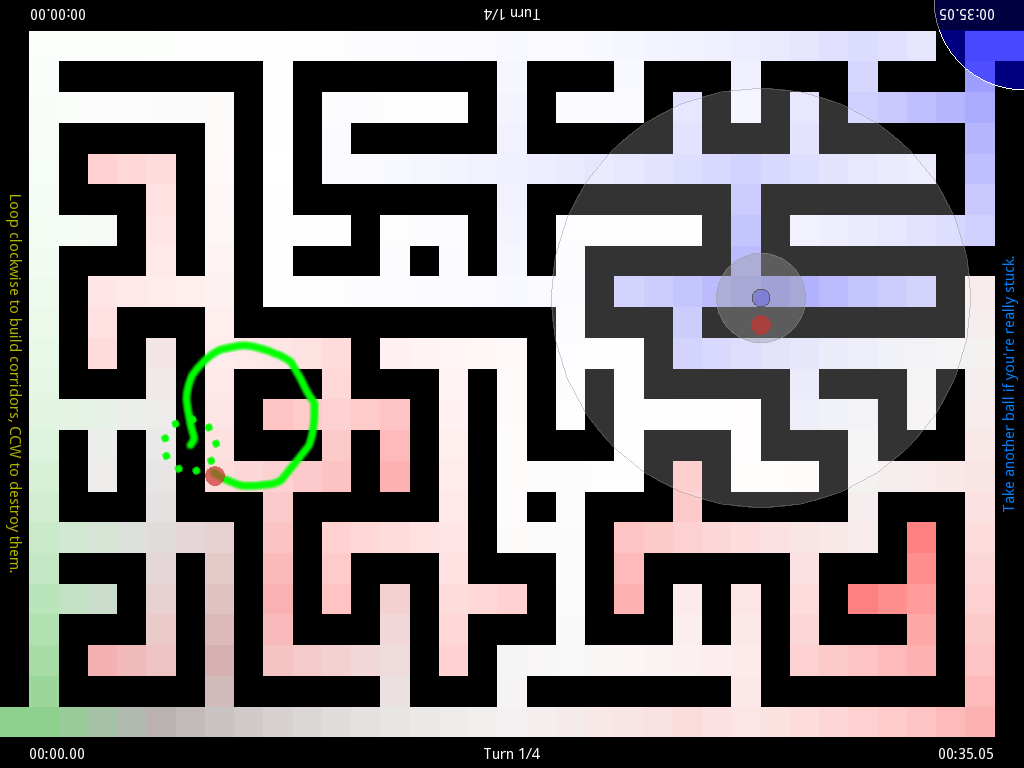
\includegraphics[width=13cm]{scsh-maze}
\caption{Screen-shot of the Maze game showing a loop being drawn and a ball
being dragged}
\label{scsh-maze}
\end{figure}

\subsubsection{Rules for the Solver}

At the beginning of a turn, the Solver must wait for five seconds to give the
Builder a chance to prepare.
Then, a blue quarter-circle, the \emph{ball source} appears in the right-hand
corner.
By touching the ball source, a small \emph{ball} is created and can be
immediately dragged out.

Around the ball is a circular area called the ball's \emph{handle}.
When the Solver touches the handle, the ball moves towards the touch with a
fixed speed, even if the touch moves, unless a maze wall prevents the movement.

Whenever a ball is touched, a large circular area forms around it.
This is the ball's \emph{zone of control}.
When a ball is not touched, the zone of control shrinks to the size of the
ball's handle.
The Builder cannot play in a zone of control.

The Solver can create additional balls at any time by “dragging them out”
of the ball source.
Against experienced opponents, it may be necessary to create a few balls and
use their zones of control to effectively limit the Builder's actions.

For each ball on the table, time is added to the Solver's \emph{clock}.
For example, if two balls are out, two seconds are added with each second of
real time.

The Solver's goal is to navigate a ball through the maze into the \emph{exit
area} in the Builder's right-hand corner of the table with as little time
on the clock as possible.

\subsubsection{Rules for the Builder}

The Builder's job is to make it hard for the Solver to reach the exit by
modifying the maze.

By drawing a clockwise loop that starts and ends on a maze wall, the wall
tile will be destroyed and replaced by a corridor.
Conversely, corridors can be destroyed (and walls built) by drawing a
counterclockwise loop.
As a loop is drawn it changes color from yellow to red or green, for destroying
and building corridors, respectively.
After finishing a loop, the builder can drag the finger across more tiles
to continue building or destroying.

There are limits to building.
At all times, all corridors must be connected to each other, and to the start
and exit of the maze.
This means that no part of the maze may be cut off, even if it does not contain
any balls.
Destroying corridors is thus limited to breaking loops and filling dead ends,
and building corridors is limited to extending or branching existing ones.
Also, the Builder cannot play in a ball's zone of control.

Usually, each maze is initially very easy, with at least one obvious way
around the maze's perimeter.
The Builder is given five seconds at the start of the turn for a chance to
block such obvious solutions.

\subsubsection{Fair play}

As the system has no way of recognizing which touch belongs to whom,
it is up to the players to only use gestures for their own role.

Most unintentional use of the opponent's gestures is prevented by the fact that
the gestures needed (drawing loops vs. dragging) are very different between the
players.

\subsection{Towers}

Towers is a two-player game in which both players are equal and each uses
only his or her half of the screen.

The point of the game is to hold off an invasion by building and upgrading
towers.
Touching empty space or a tower triggers a menu with options to build, upgrade,
and/or sell a tower.

While the above instructions is all players initially need to know to play the
game, the next section describes the mechanics further.

\subsubsection{Game Control and Mechanics}

On each player's side is a white strip called the \emph{home area}. The amount
of a player's money is shown on the home area.
Small circular entities called \emph{critters} are spawned in the middle of the
screen and move towards each player's home area.
Each “generation” of critters has a higher amount of \emph{hit points (HP)}
than the previous one, and critters are created in shortening intervals.
This makes the game progressively more difficult as time passes.

\begin{figure}[hb]
    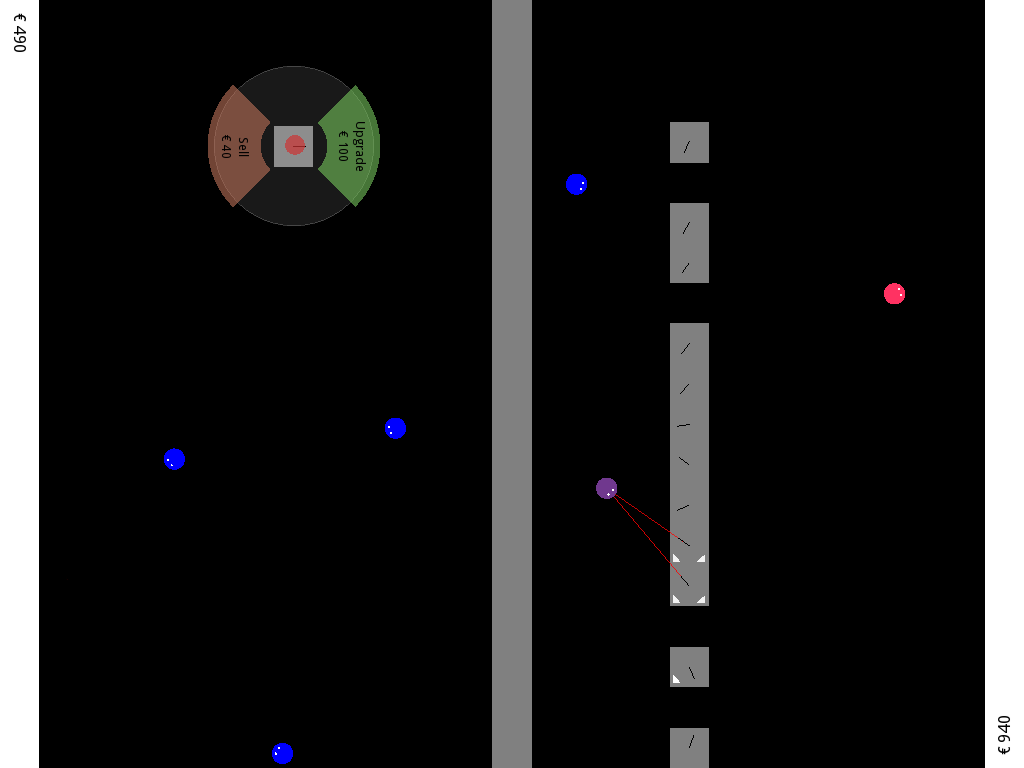
\includegraphics[width=13cm]{scsh-towers}
\caption{Screen of the Towers game showing an upgrade menu, critters and towers.
        Two towers that were upgraded for a greater range are firing at a critter.}
\hspace{1em}
\label{scsh-towers}
\end{figure}

Once a critter reaches the home area, the player's money is continually
decreased and the critter loses its HP, until the HP drops to zero and the
critter is eliminated.
Critters change color from blue to red as they lose HP.

To prevent critters from reaching the home area, a player can build
\emph{towers}.
Touching the empty area of the screen opens a circular menu with one option,
Build, located away from the player.
Dragging the finger towards this option triggers a circular progress bar that
gradually fills up, consuming some of the player's money.
When the progress bar is full, a tower is built.
If the finger is released while the tower is building, the progress bar
starts gradually draining.
If allowed to fully drain, the building is cancelled.
Touching the tower site while the progress bar is draining resumes building.

A tower fires shots at critters close to it.
Each shot removes some of the target critter's HP.
When a critter's HP drops to zero this way, the critter is removed and some
money is awarded to the owner of the tower.
Once a tower fires, it “remembers” the \emph{target critter}, and will keep
shooting at it until the critter is removed from game or moves out of range.
If a tower has no target critter, one is selected.
Heavily damaged critters, and those close to the tower, are favored as targets.
The game does not prevent “stealing kills” by shooting critters in the
opponent's half of the screen, however this practice requires towers with a
long range and a lack of better targets at the player's own field, so it is
difficult to accomplish.
Nevertheless, money is always awarded to the owner of the tower that deals the
“finishing blow”.

Critters cannot pass through towers, which allows the player to create a maze,
forcing critters to go along a longer path and creating more
opportunities to hit them.
Similarly to the Maze game, a player cannot build a tower that blocks off a
part of the area completely.
The critters generally follow the shortest path to a player's home area,
but their movements are slightly randomized.

When a player touches an existing tower, a circular \emph{upgrade menu},
similar to the one displayed for building a tower, is shown.
This menu contains two options: \emph{Upgrade} and \emph{Sell}.
In addition to the menu, whenever a tower is being touched, its range
is visualized as a circle.

Selecting Upgrade causes a tower upgrade, which is similar to building a tower,
except the tower is not destroyed if the upgrade is cancelled.
Upon completion of an upgrade, the tower's \emph{level} increases, which
increases the tower's range and causes the tower to fire more rapidly and deal
more damage with each shot.
A tower's level is indicated graphically by small white triangles or a square
on the tower.
After a maximum level is reached, a tower may not be upgraded further.

Selecting the Sell option on the upgrade menu causes the tower to disappear
and some money to be returned to the player.

When a player is out of money, any building or upgrading is suspended.
If a player goes in debt (due to critter infestation of the home area), towers
are automatically sold until the debt is paid off.
If there are no towers to sell, the player loses the game.
The player that does not lose – or would lose after his or her opponent – wins.

(It may be noted that once a player starts losing towers due to debt, there is
usually no way to stop losing them.
The automatic selling of towers is a way of taking the “tower capital” into
account when determining win and loss, and providing a final “your empire is
crumbling” animation.)

Figure~\ref{scsh-towers} shows the game screen and visual elements.

\subsection{Replay}

All games are recorded. Whenever a game is run, a log file is created in the
current directory.
Using the replay script, a recorded game can be played back by giving the log
filename as a command line parameter.
The replay script must be started with the same parameters (e.g. window
size) as the original game.
Touching the replay window allows the user to slow down or speed up the replay.
A label showing the current speed is shown when the window is touched.

Replaying allows the user to analyze past games and study players' behavior and
strategies.

\end{document}
